\chapter{Physics Beyond The Standard Model}
\label{chap:bsm}

%\epigraph{\textit{All models are wrong, but some are useful.}}{--George Box}
\epigraph{\textit{The only consolation he drew from the present chaos was that his theory managed to explain it.}}{--Thomas Pynchon, \textit{V.}}

%As seen in the previous section, the SM is not an adequate theory to describe the entirety of the
%observable phenomena in the universe. However, it is still exceedingly useful in describing
%the... and predicting...
%
%There are a multitude of theories describing phsyics beyond the standard model, each attempting to
%explain the shortcomings of the SM either in part or in whole, though none have so far appeared to be
%useful in the sense of being able to extend our current understanding of the the universe by providing
%objectively falsifiable prediction.


%%%%%%%%%%%%%%%%%%%%%%%%%%%%%%%%%%%%%%%%%%%%%%%%%%%%%%%%%%%%%%%%%%%%%%%%%%%%%
%%%%%%%%%%%%%%%%%%%%%%%%%%%%%%%%%%%%%%%%%%%%%%%%%%%%%%%%%%%%%%%%%%%%%%%%%%%%%
%%%%%%%%%%%%%%%%%%%%%%%%%%%%%%%%%%%%%%%%%%%%%%%%%%%%%%%%%%%%%%%%%%%%%%%%%%%%%
%
% GENERAL
%
%%%%%%%%%%%%%%%%%%%%%%%%%%%%%%%%%%%%%%%%%%%%%%%%%%%%%%%%%%%%%%%%%%%%%%%%%%%%%
%%%%%%%%%%%%%%%%%%%%%%%%%%%%%%%%%%%%%%%%%%%%%%%%%%%%%%%%%%%%%%%%%%%%%%%%%%%%%
%%%%%%%%%%%%%%%%%%%%%%%%%%%%%%%%%%%%%%%%%%%%%%%%%%%%%%%%%%%%%%%%%%%%%%%%%%%%%
\cite{2HDMPheno,EWSBMSSM,SUSYPrimer,LightStopsHiggs}
\cite{EWSBProbeRho,PDGRef}
\cite{ColemanMandula,WessZuminoModel,HaagSUSY}

As seen in Section~\ref{sec:final_sm_description}, the SM provides an incredible toolkit
from which the majority of the observed physical phenomena can be described.
As we saw, however, there are several glaring open questions whose answers must be pursued
if we are to truly understand the underlying nature of the Universe.
Given the scope of these open questions, and the apparent inconsistencies exposed by the Hierarchy Problem,
their solutions are all but guaranteed to further revolutionize our view of the Universe.
As a result, there have been a multitude of proposals of new theories of particles and fields over the preceding decades that attempt
to solve some of these remaining mysteries.


With the discovery of the 125\,GeV Higgs boson, the physics community is seemingly
on the verge of gaining further insight into the nature of these problems.
Any new source of physics beyond the SM (BSM) will necessarily have much to say
about the electroweak and Higgs sectors of the SM,
especially in view of the Hierarchy Problem's hinting at the electroweak scale
being so near the portal to new physics.
These sectors tightly constrain the forms that BSM physics can take, as well, if they
are to remain consistent with the precise confirmation of the SM predictions
over the past 50-60 years.
One such constraint, a beautiful result of the electroweak theory and one that
is fundamental to the nature of EWSB, is that of the $\rho$ parameter of the SM,
defined in Equation~\ref{eq:rho_sm}.
The precise equality of Equation~\ref{eq:rho_sm} can be seen to hold by using the relationships
between the electroweak gauge mixings and couplings in Equations~\ref{eq:weinberg_angles} and \ref{eq:gauge_boson_masses}.
The $\rho = 1$ equality holds to very high precision even when including higher order
corrections to the gauge boson masses and interactions, a fact that his been verified
by precision measurements~\cite{EWSBProbeRho,PDGRef}.

\begin{align}
    \rho = \frac{
                M_W
            }
            {
                M_Z \cos \theta_W
            }
        \underset{\text{\tiny{SM}}}{=} 1
    \label{eq:rho_sm}
\end{align}
The requirement that $\rho = 1$ restricts the form any new BSM physics attempting to alter
the electroweak sector can take.
In fact, the relation holds for Higgs sectors that are more complex than the minimal one
predicted by the SM.
It can be shown that extended Higgs sectors, composed of \textit{multiple} scalar Higgs doublets
so long as their \SUtwo~and \Uone~gauge structure satisfies the fundamental relation in Equation~\ref{eq:rho_general},
\begin{align}
    \rho = \frac{
                \sum\limits_{i = 1}^n \, \left[ T_{3,i} \left( T_{3,i} + 1 \right) - Y_i^2 \right ] v_i
            }
            {
                \sum\limits_{i=1}^n \, 2 Y_i^2 v_i
            },
    \label{eq:rho_general}
\end{align}
where $n$ runs over the number of scalar Higgs doublets in the theory, $T_{3}$ and $Y$ are the \SUtwo~and \Uone~gauge
quantum numbers, respectively, associated with each doublet, and the $v$ are each of their vacuum expectation values.
In the SM, with only the single Higgs doublet having $Y = 1/2$ and $T_3 = 1/2$ (Table~\ref{tab:sm_content}),
the equality clearly holds.

The possibility that the Higgs sector may be more complex without disrupting strict relationships
predicted very cleary by the SM has led to the development of many fields of research.
One such potential for BSM physics is the class of theories that minimally extend the
Higgs sector by only including a single additional scalar double ($n = 2$ in Equation~\ref{eq:rho_general}).
Such theories are referred to as Two Higgs-Doublet Models (`2HDMs'), and their
phenomenology is rich~\cite{2HDMPheno}.
The two Higgs doublets are typically referred to as `$H_u$' and `$H_d$', where the subscripts
indicate to which component of the \SUtwo~fermions they couple and give mass, are complex scalar
fields with eight degrees of freedom.
In these models, the three degrees of freedom needed for the $W^{\pm}$ and $Z$ bosons
to acquire mass after EWSB leave open five additional degrees of freedom.
As a result, 2HDMs are characterized by an extended Higgs sectors in which there are \textit{five
physical massive Higgs bosons}: two neutral components ($h^0$ and $H^0$), one netural pseudoscalar particle ($A^0$),
and two that are electrically charged ($H^{\pm}$).
The neutral component $h^0$ is typicaly considered to be lightest Higgs boson and is identified as the
125\,GeV boson discovered in 2012.
Other than this assumption on $h^0$, the mass spectrum of these five Higgs bosons and their 
phenomenology is dependent on the specific instantiation of the 2HDM in question.
As it turns out, one of the most promising all-encompassing theories of new physics,
Supersymmetry (SUSY), is a 2HDM.
Section~\ref{sec:susy} provides a brief introduction to SUSY that will be relevant
as background to the analyses presented in Chapters~\ref{chap:search_stop} and \ref{chap:search_hh}.

%%%%%%%%%%%%%%%%%%%%%%%%%%%%%%%%%%%%%%%%%%%%%%%%%%%%%%%%%%%%%%%%%%%%%%%%%%%%%
%%%%%%%%%%%%%%%%%%%%%%%%%%%%%%%%%%%%%%%%%%%%%%%%%%%%%%%%%%%%%%%%%%%%%%%%%%%%%
%%%%%%%%%%%%%%%%%%%%%%%%%%%%%%%%%%%%%%%%%%%%%%%%%%%%%%%%%%%%%%%%%%%%%%%%%%%%%
%
% SUSY
%
%%%%%%%%%%%%%%%%%%%%%%%%%%%%%%%%%%%%%%%%%%%%%%%%%%%%%%%%%%%%%%%%%%%%%%%%%%%%%
%%%%%%%%%%%%%%%%%%%%%%%%%%%%%%%%%%%%%%%%%%%%%%%%%%%%%%%%%%%%%%%%%%%%%%%%%%%%%
%%%%%%%%%%%%%%%%%%%%%%%%%%%%%%%%%%%%%%%%%%%%%%%%%%%%%%%%%%%%%%%%%%%%%%%%%%%%%
\section{Supersymmetry}
\label{sec:susy}

SUSY is a theoretical framework that allows for the fermionic (spin-1/2) and bosonic (spin-1)
fields to mix.
That is, it allows one to relate the fields typically associated with matter with those
typically associated with the forces and interactions by introducing the SUSY generators $Q$ that
allow to interchange a fermion with a boson:
\begin{align}
    Q \ket{\text{fermion}} = \ket{\text{boson}}, \hspace{1cm} Q \ket{\text{boson}} = \ket{\text{fermion}}
    \label{eq:susy_operator}
\end{align}
As spin is fundamentally associated with a \textit{spacetime} symmetry, the notion 
that the fermions and bosons could be related in such a way was famously forbidden
by the `no-go' theorem of Coleman and Mandula~\cite{ColemanMandula} which stated that the
the structure
of the SM was maximal.
That is, there could be no other form for the mixing of spacetime and internal
symmetries other than by the direct product formulation of the SM: $\mathcal{P} \times$\SUthree$_C \times $ \SUtwo$_L \times$ \Uone$_{Y}$.
The work of Ref.~\cite{HaagSUSY} provided a way out, however, and was able to show
that spacetime and internal symmetries could mix more generally if the generators, $Q$, were \textit{fermionic} --- with spin no greater than 1/2 --- rather than
bosonic, as is the case in the SM.
That four dimensional SUSY was shown to be possible, and that matter-type fields and particle-type fields
are possibly two sides of a more fundamental coin, is an exciting proposition and opened
up SUSY as one of the more enticing avenues for the search for new physics.

SUSY proposes that each SM particle be partnered with a new particle, its `super-partner', whose spin differs
by 1/2 unit \textit{less} than the SM partner.
These super-partners are then grouped into the `super-multiplets'
on which the SUSY algebra operates.
%At its core, then, SUSY introduces `super-multiplets' on which the SUSY algebra
%operates.
The structure of the super-multiplets is as follows,

\begin{align}
    \underbrace{\begin{pmatrix}
        f_{\small{1/2}} \\
        \tilde{\phi}_0
    \end{pmatrix}}_{\substack{\text{Chiral} \\ \text{Supermultiplet}}}
    \hspace{1cm}
    \underbrace{\begin{pmatrix}
        V_1 \\
        \tilde{V}_{1/2}
    \end{pmatrix}}_{\substack{\text{Gauge} \\ \text{Supermultiplet}}}
    \hspace{1cm}
    \begin{matrix}
        \begin{cases}
            \begin{tabular}{l l}
                $f_{1/2}$~: & \text{Spin-1/2 Weyl fermion} \\
                $\tilde{\phi}_0$~: & \text{Complex scalar} 
            \end{tabular}
        \end{cases} \\
        %\hspace{1.3cm}
        \begin{cases}
            \begin{tabular}{l l}
                $V_1$~: & \text{Spin-1 boson} \\
                $\tilde{V}_{1/2}$~: & \text{Spin-1/2 Weyl fermion}
            \end{tabular}
        \end{cases}
    \end{matrix},
    \label{eq:susy_multiplets}
\end{align}
%This structure is illustrated in Equation~\ref{eq:susy_multiplets}.
with the spin-1/2 fermions of the SM being paired with their scalar SUSY partner in
the `chiral super-multiplets' and 
the spin-1 gauge bosons of the SM being paired with fermionic SUSY partners
in the `gauge super-multiplets'.
The newly added SUSY particles are labelled with a `$\sim$' to distinguish them relative to the SM particles.
The structure of these multiplets implies a \textit{doubling} of the particle content
of the SM, which has broad consequences on the ways that SUSY can potentially manifest itself and necessarily implies a rich
phenomenology.

The additional particle content implied by a minimal instantiation of SUSY, referred
to as the Minimally Supersymmetric SM (`MSSM'), is presented in Table~\ref{tab:mssm_particles}.
The squarks and sleptons are the SUSY partners of the quarks and leptons.
The neutralinos and charginos are the electroweak partners to the SM electroweak gauge bosons.
It should be noted that the squarks and sleptons are scalar, so they are inherently not chiral:
the subscripts $L$ and $R$ appearing in their name refer to the SM particle to which they are partnered.
The $f_L$ and $f_R$ can generally mix to form the physical fields, $f_1$ and $f_2$; however, it is generally assumed
that only those in the third generation mix appreciably.
The physical fields have subscripts $\{1,2,...\}$ with the lower numbers referring to the particles
with the lower mass.
For example, $m_{\tilde{t}_1} < m_{\tilde{t}_2}$.
Table~\ref{tab:mssm_particles} also shows that the SUSY partners to the two Higgs doublets, $\tilde{H}^0_d$ and $\tilde{H}^{0}_u$, mix with the
SUSY partners of the electroweak gauge bosons.
The structure of the mixing of the fundamental gauge eignstates in the electroweak sector of SUSY
leads to complicated mass heirarchies of the $\tilde{\chi}^0$ and $\tilde{\chi}^{\pm}$ particles, meaning that searches
for these particles will be inherently challenging.

In most MSSM scenarios, it is assumed that an additional symmetry, referred to as `$R$-parity', exists
and that the SM particles have $R$-parity quantum number $+1$ and the SUSY particles $-1$.
For the types of SUSY relevant to the present thesis, it is assumed that $R$-parity is absolutely conserved.
SUSY scenarios having conserved $R$-parity are referred to as `$R$-parity conserving (RPC) SUSY' scenarios.\footnote{
Alternatively, those with non-conserved $R$-parity are referred to as $R$-parity violating and are referred
to as `RPV SUSY' scenarios.
}
RPC SUSY scenarios imply that the lightest supersymmetric particle (`LSP') must be absolutely stable.
The current lack of any directly observed additional particle content in the Universe implies that the LSP, while stable,
must also be weakly interacting and electrically neutral.
As a result, the LSP is typically taken to be $\tilde{\chi}^0_1$.
One major consequence, then, of RPC SUSY is that it provides a natural candidate for WIMP-like\footnote{
The abbreviation `WIMP' stands for `weakly-interacting massive particle'.
} DM via the $\tilde{\chi}^0_1$ fermion.

\begin{table}[!htb]
    \begin{center}
        \caption{
            Particle content of the MSSM.
        }
        \label{tab:mssm_particles}
        \begin{tabular}{c | c | c | c | c}
        %\begin{tabular}{c | c | c | Sc | Sc}
        \hline
        \hline
            \textbf{Names} & \textbf{Spin} & \textbf{R-Parity} & \textbf{Gauge Eigenstate} & \textbf{Mass Eigenstate} \\
            \hline
            \multirow{3}{*}{Squarks} & \multirow{3}{*}{0} & \multirow{3}{*}{$-1$} & $\tilde{u}_L, \,\tilde{u}_R, \, \tilde{d}_L, \, \tilde{d}_R$ & same  \\
                                                & & & $\tilde{c}_L, \,\tilde{c}_R, \, \tilde{s}_L, \, \tilde{s}_R$ & same  \\
                                                & & & $\tilde{t}_L, \,\tilde{t}_R, \, \tilde{b}_L, \, \tilde{b}_R$ & $\tilde{t}_1,\,\tilde{t}_2,\,\tilde{b}_1,\,\tilde{b}_2$  \\
            \hline
            \multirow{3}{*}{Sleptons} & \multirow{3}{*}{0} & \multirow{3}{*}{$-1$} & $\tilde{e}_L,\,\tilde{e}_R,\,\tilde{\nu}_e$ & same \\
                & & & $\tilde{\mu}_L,\,\tilde{\mu}_R,\,\tilde{\nu}_{\mu}$ & same \\
                & & & $\tilde{\tau}_L,\,\tilde{\tau}_R,\,\tilde{\nu}_{\tau}$ & $\tilde{\tau}_1,\,\tilde{\tau}_2,\,\tilde{\nu}_{\tau}$ \\
            \hline
            Neutralinos & $1/2$ & $-1$ & $\tilde{B}^0,\,\tilde{W}^0,\,\tilde{H}^0_u,\,\tilde{H}^0_d$ & $\tilde{\chi}^0_1,\,\tilde{\chi}^0_2,\,\tilde{\chi}^0_3,\,\tilde{\chi}^0_4$ \\
            \hline
            Charginos & $1/2$ & $-1$ & $\tilde{W}^{\pm},\,\tilde{H}^+_u,\,\tilde{H}^-_d$ & $\tilde{\chi}^{\pm}_1,\,\tilde{\chi}^{\pm}_2$ \\
            \hline
            Gluino & $1/2$ & $-1$ & $\tilde{g}$ & same \\
            \hline
            \hline
            Higgs Bosons & 0 & $+1$ & $H_u^0,\,H_d^0,\,H_u^+,\,H_d^-$ & $h^0,\,H^0,\,A^0,\,H^{\pm}$  \\
        \hline
        \hline
        \end{tabular}
    \end{center}
\end{table}

An additional consequence of SUSY is that the Hierarchy Problem, described in Section~\ref{sec:final_sm_description},
can potentially be resolved entirely.
This can be seen by computing the additional loop contributions to the Higgs mass corrections arising as a result of fundamental scalars.
The additional loops from such scalar particles are illustrated in Figure~\ref{fig:higgs_mass_correction_stop}.
\begin{figure}[!htb]
    \begin{center}
        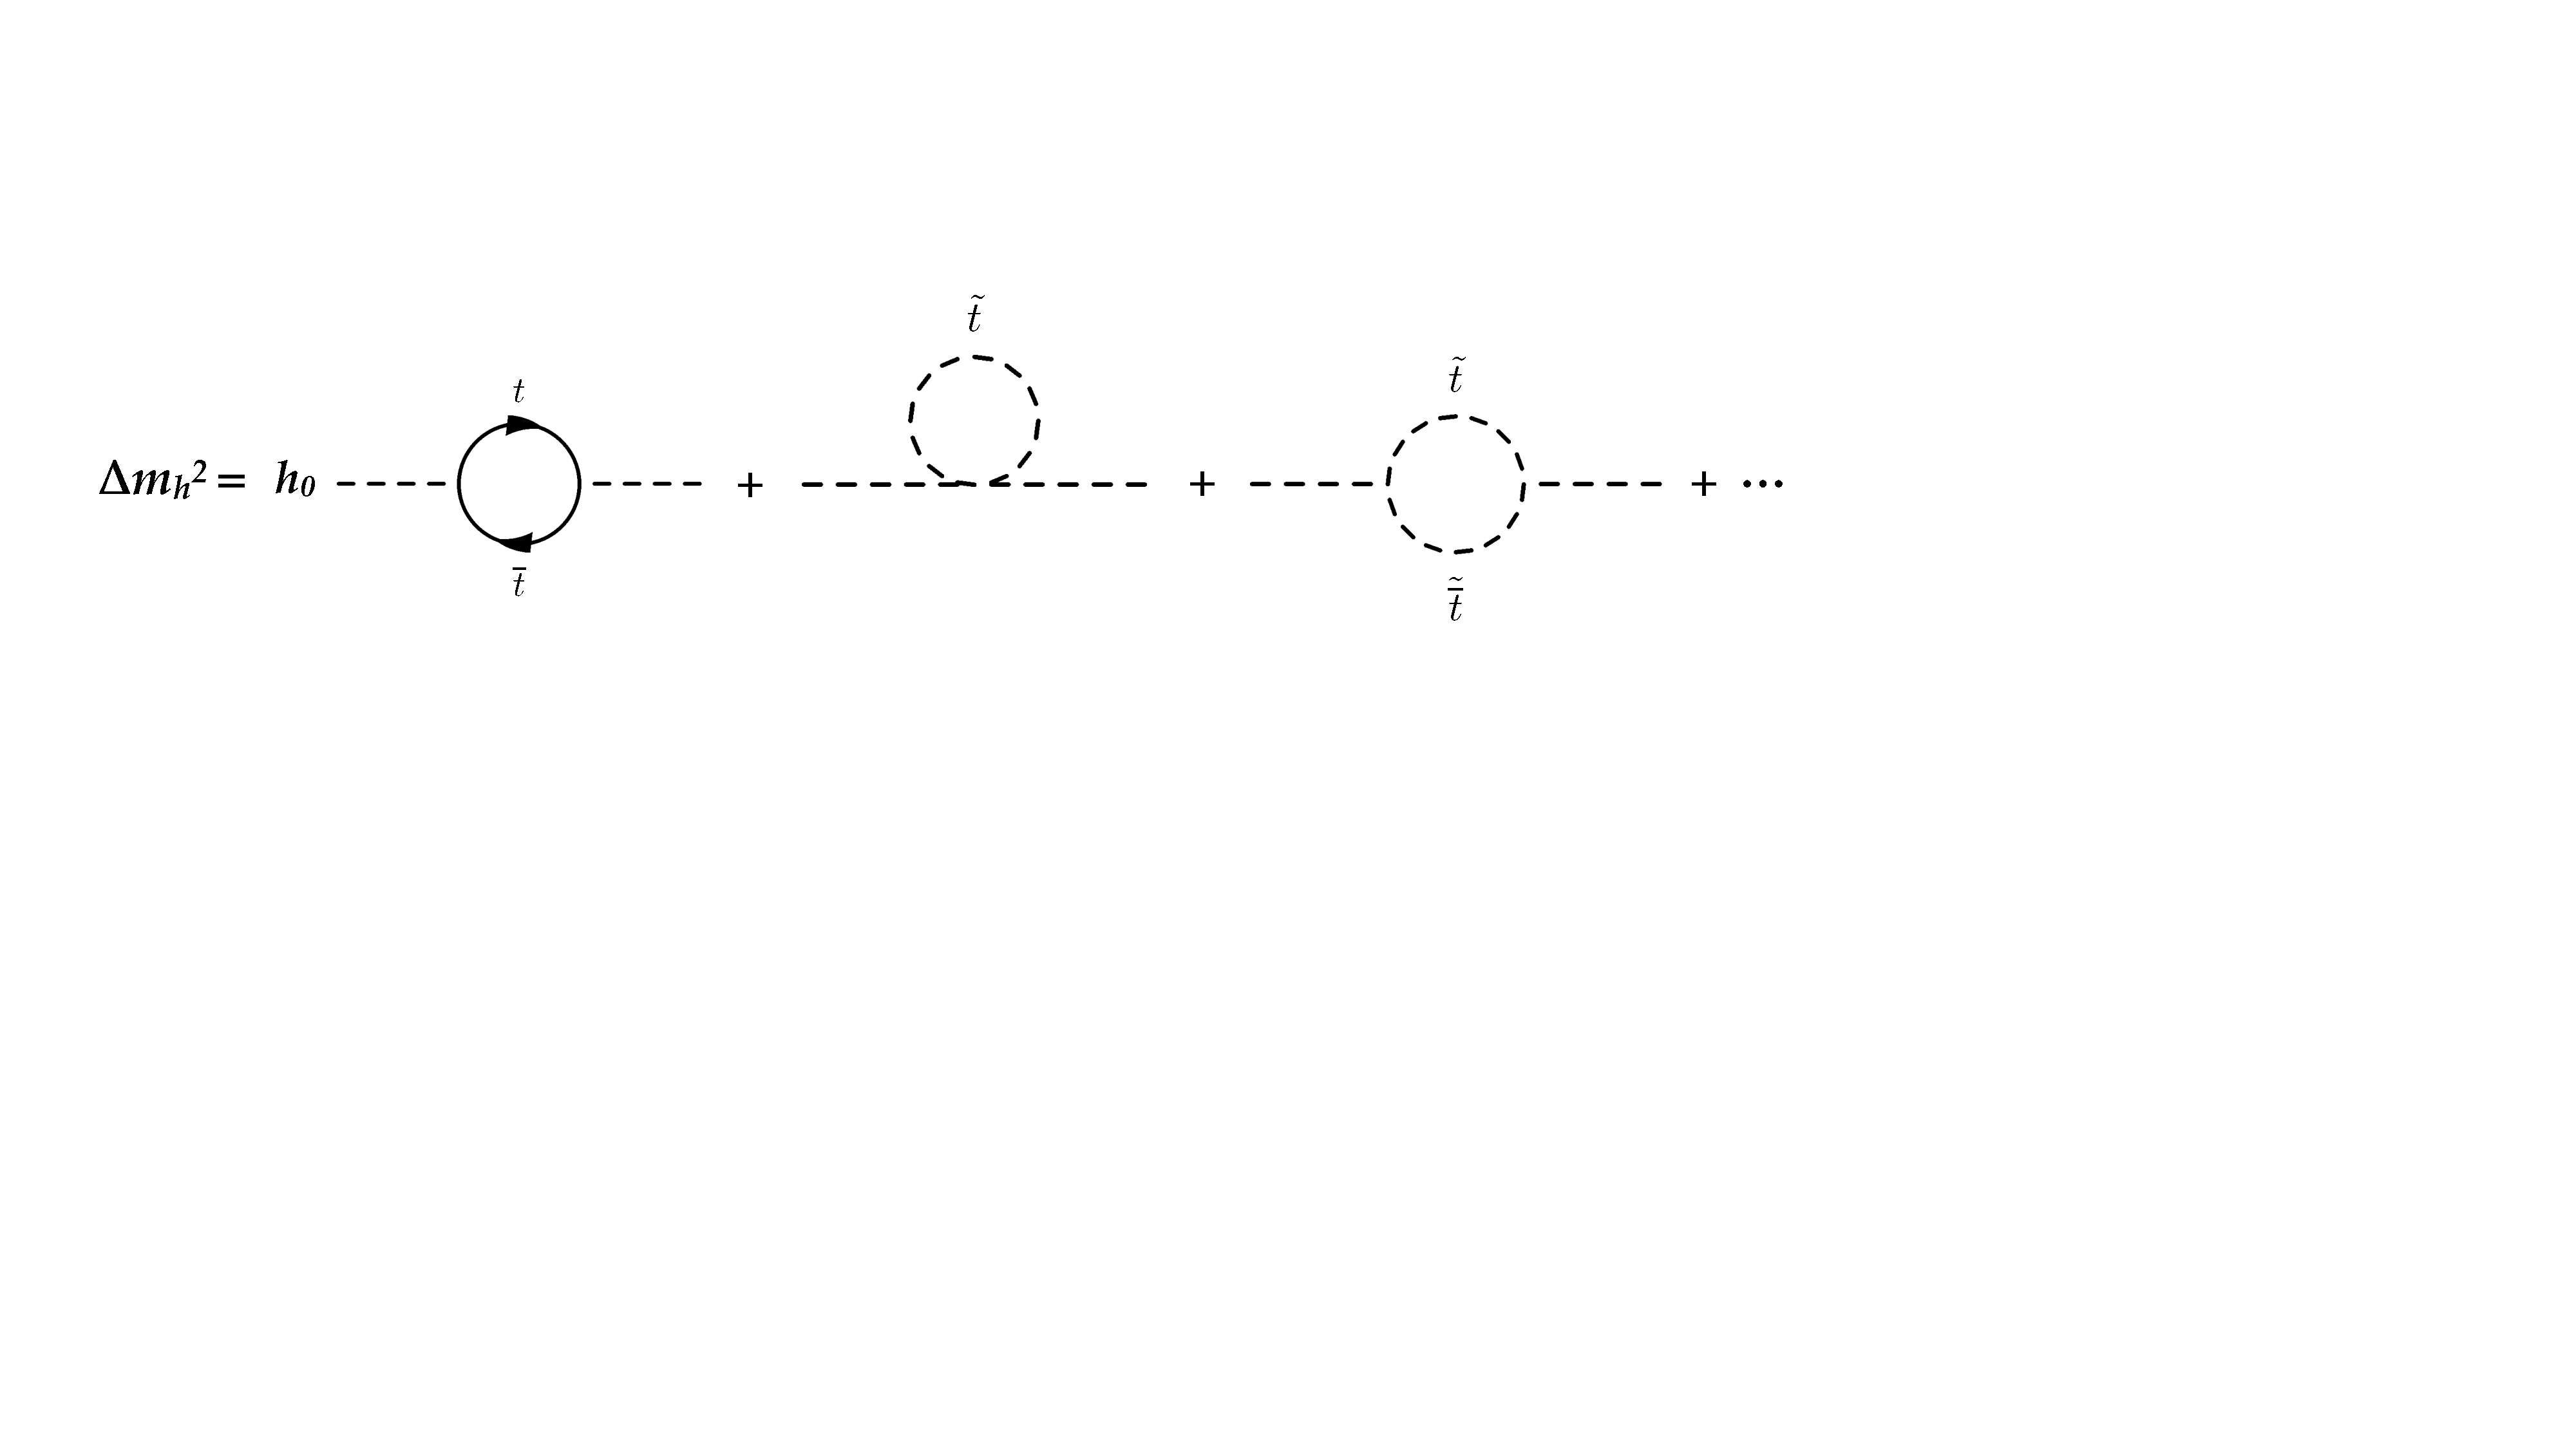
\includegraphics[width=0.9\textwidth]{figures/higgs_corr/higgs_mass_corrections_stopPDF}
        \caption{
            Loop contributions to the higher-order computation of the Higgs mass as a result of the SM top-quark, $t$,
            and its scalar superpartner, $\tilde{t}$.
        }
        \label{fig:higgs_mass_correction_stop}
    \end{center}
\end{figure}
The scalar contributions take the form of Equation~\ref{eq:higgs_corr_susy},
\begin{align}
    \left( \Delta m_h^2 \right)_{S} = \frac{\lambda_S}{16 \pi^2} \left[ 2 \Lambda^2 - \mathcal{O} \left( m_S^2 \ln \left( \frac{\Lambda}{m_S} \right) \right) \right],
    \label{eq:higgs_corr_susy}
\end{align}
where $m_S$ is the scalar mass and $\lambda_S$ is its Yukawa-type Higgs coupling parameter.
These scalar loop corrections are seen to suffer the same type of quadratic divergence
as in the case of Equation~\ref{eq:higgs_divergence} but they enter \textit{with an opposite overall sign}.
Combining the fermionic and scalar loops from particles in the same chiral super-multiplet leads
to an overall correction of the form shown in Equation~\ref{eq:higgs_corr_fixed}:
\begin{align}
    \Delta m_h^2 \underset{\text{w/ SUSY}}{\propto} \left( m_f^2 - m_S^2 \right) \ln \left( \frac{\Lambda}{m_S} \right) + 3 m_f^2 \ln \left( \frac{m_S}{m_f} \right) + \mathcal{O} \left( \frac{1}{\Lambda^2} \right)
    \label{eq:higgs_corr_fixed}
\end{align}
The remarkable feature that Equation~\ref{eq:higgs_corr_fixed} shows is that if SUSY is \textit{exact}, that is if the particles within the same supermultiplet 
enter with the same mass ($m_f = m_S$) and have the same couplings ($y_f = \lambda_f$), then the problematic divergence underlying the Hierarchy Problem
disappears!
This is a very suggestive result that we immediately know, however, not to be the case
in reality given the fact that
the observation of additional particles with the exact same masses of the known SM particles would
have been made ages ago.
If SUSY is to exist as described by the MSSM (Table~\ref{tab:mssm_particles}) it must then
be a \textit{broken symmetry} wherein the masses of the SUSY partners are larger than
their SM counterpart --- large enough such that they would have escaped experimental detection
in high energy particle colliders up until the present day.

As mentioned in Section~\ref{sec:sm_shortcomings}, however, the experimental observation of a relatively
light Higgs boson is suggestive of new physics entering at the electroweak scale.
If this assumption is taken to heart, and if SUSY is to explain away the Hierarchy Problem, among other things,
then the implied cancellation in Equation~\ref{eq:higgs_corr_fixed} should still hold, at least approximately.
This implies that the masses of at least the lightest SUSY partners cannot be too large
and should be no larger than $\mathcal{O}(\TeV)$,
\begin{align}
    |m_f^2 - m_S^2| \le \mathcal{O}(\text{TeV}^2).
    \label{eq:tev_susy}
\end{align}
As the leading contribution to the loop corrections to the Higgs mass arise due to the SM top-quark loops,
the relation in Equation~\ref{eq:tev_susy} implies that the scalar SUSY partners to the top-quark should
not be much larger than $\mathcal{O}(\TeV)$.
If this is true, that TeV-scale SUSY partners to the SM top-quark exist, they should in-principle
be able to be produced at the center-of-mass collision energies available at the LHC.

The above discussion places a fundamental importance on the SUSY partner to the SM top quark.
Apart from simply producing them directly within the $pp$ collisions at the LHC,
their presence may be observed \textit{indirectly}.
In Section~\ref{sec:sm_successes} the fundamental importance of the production of Higgs boson
pairs was introduced, with the leading production mechanisms in the SM indicated
by the diagrams in Figure~\ref{fig:hh_feynman}.
If the SUSY partner to the top-quark exists, and is not too heavy as suggested by Equation~\ref{eq:tev_susy},
then it may contribute additional diagrams leading to final state
pairs of Higgs bosons.
Potential, additional single-loop contributions of this type are illustrated
in Figure~\ref{fig:hh_stops}.
Depending on the exact configuration of the MSSM, then, the presence of the scalar partner
of the SM top-quark could potentially lead to non-SM values for the Higgs self-coupling parameter $\lambda$ and
also to \textit{enhanced} rates of Higgs boson pairs
being produced at the LHC~\cite{LightStopsHiggs}.
This latter fact is illustrated in Figure~\ref{fig:hh_sigma_stops}, which shows the general
trend --- relatively independent of the MSSM configuration --- that low-mass scalar partners to the top-quark
can lead to appreciable increases in the Higgs boson pair-production cross-section.
This is an interesting consequence of the scalar partners of the top-quark being relatively
light.
Given the exceedingly low SM-predicted cross-section for Higgs boson pair-production at the LHC,
observation of Higgs boson pairs in the current and next runs of the LHC may imply that SUSY
is indeed hiding near the electroweak scale.

\begin{figure}[!htb]
    \begin{center}
        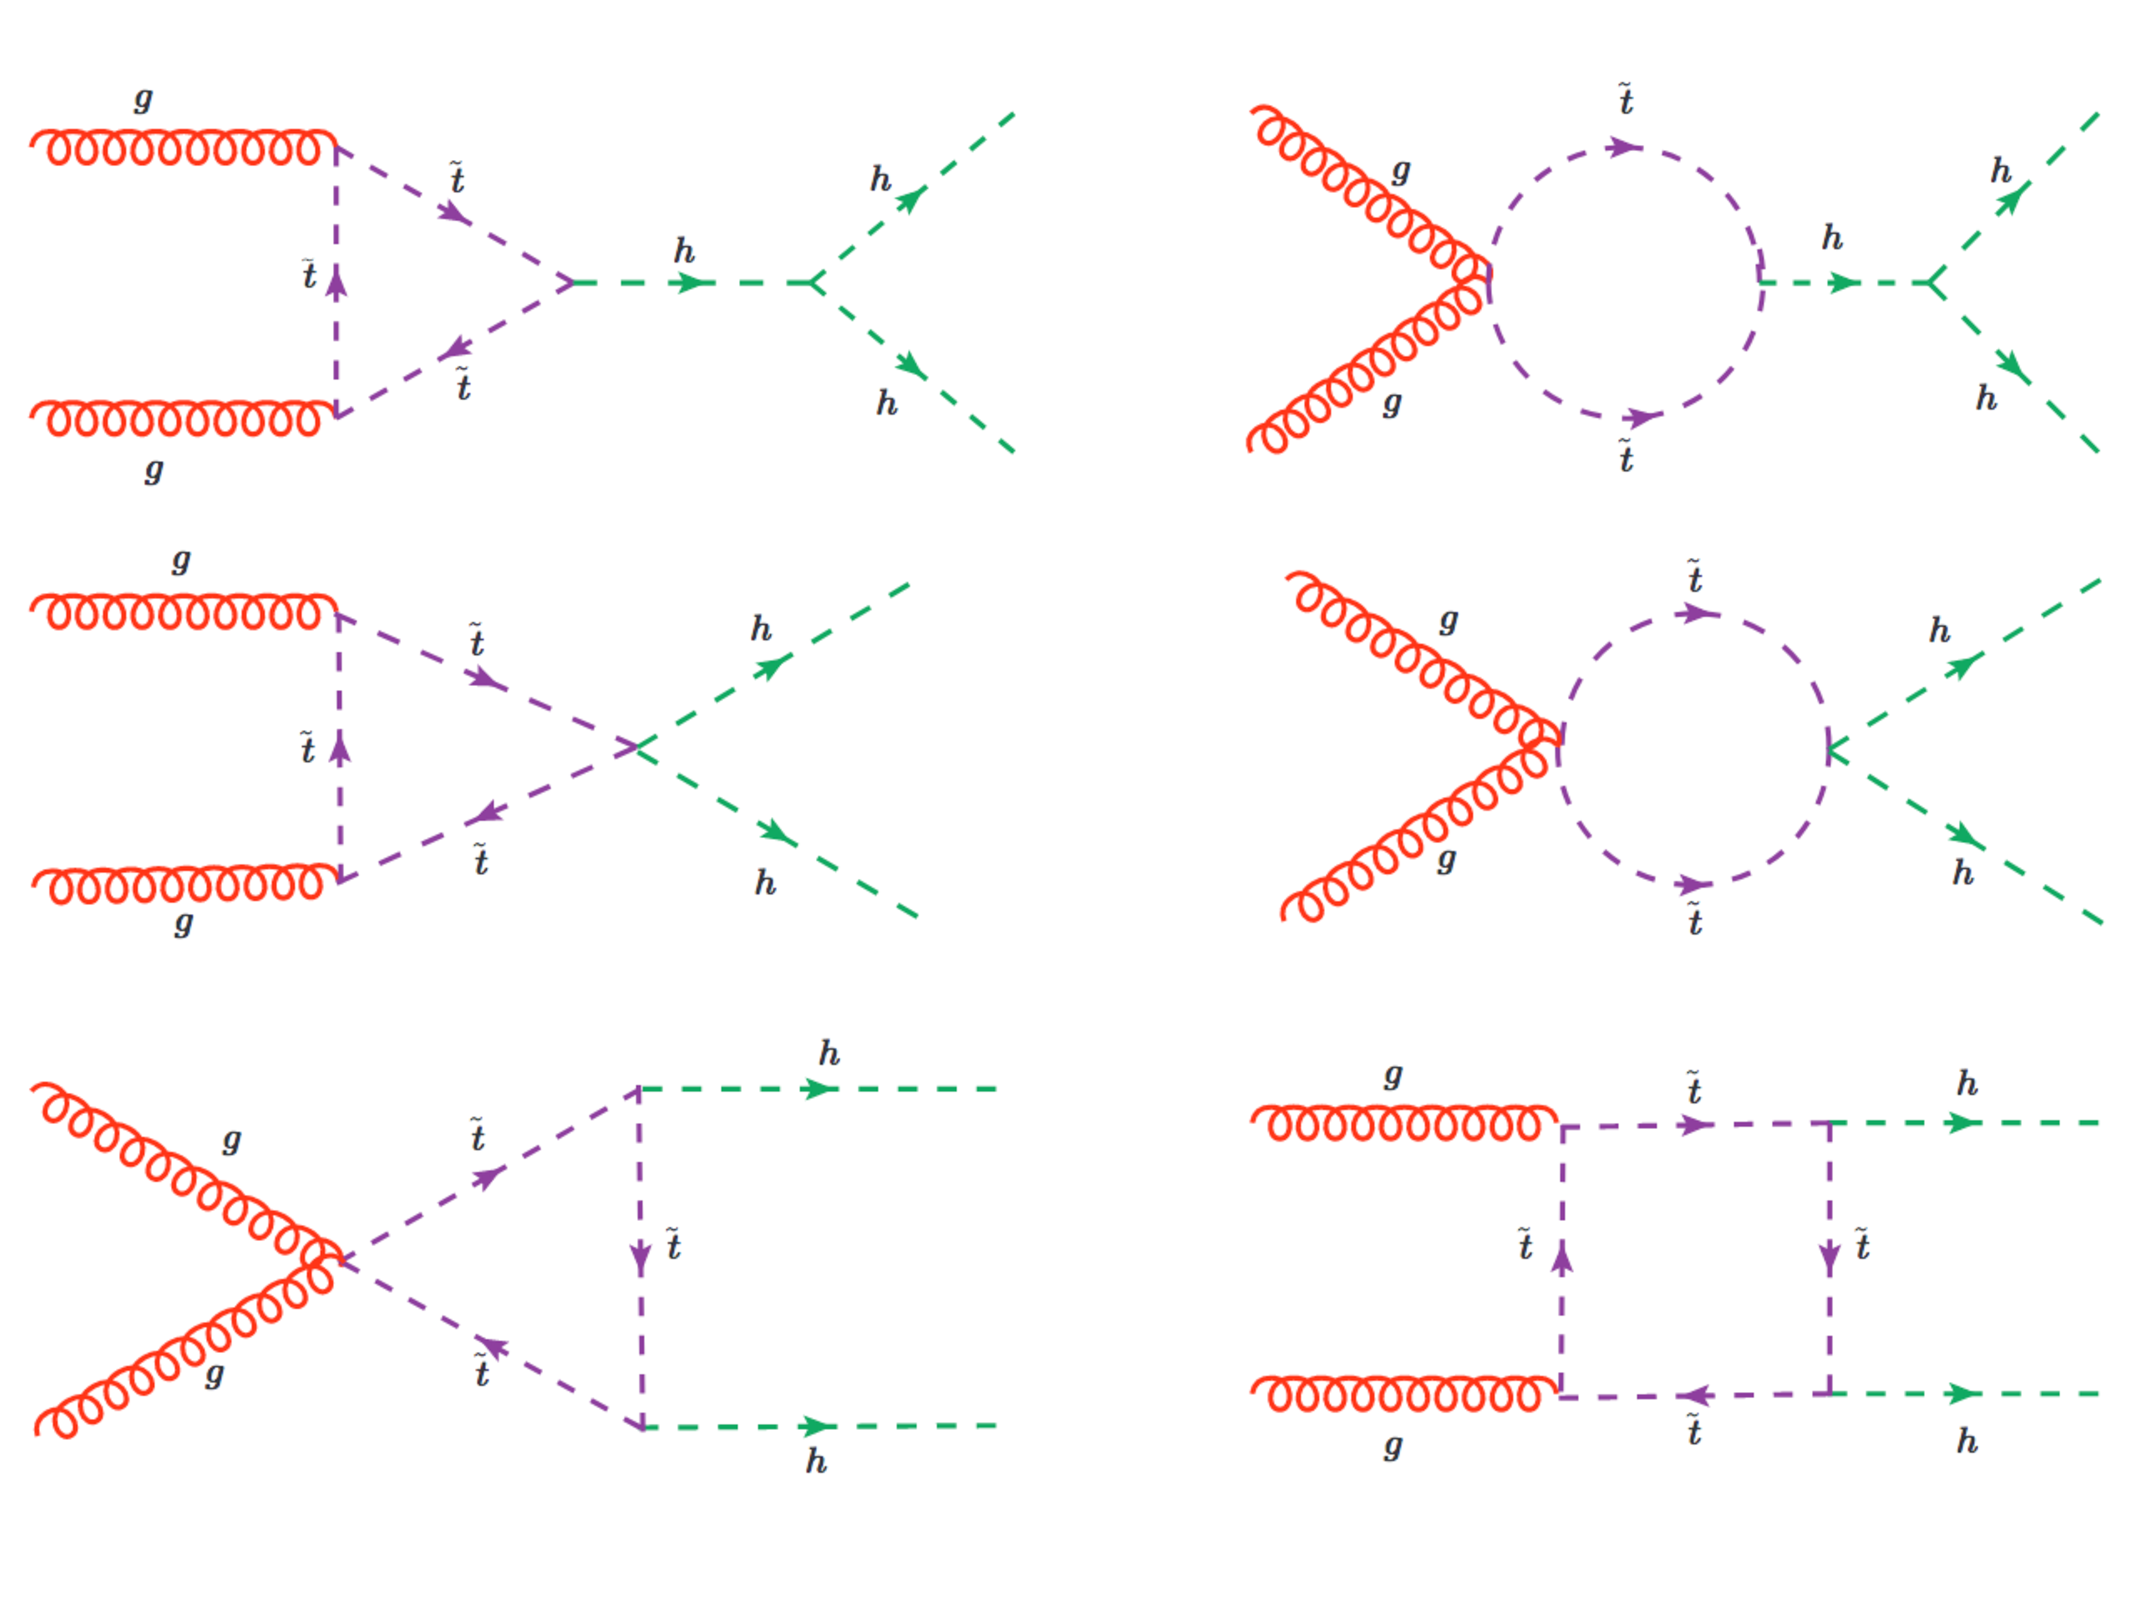
\includegraphics[width=0.95\textwidth]{figures/higgs_corr/hh_stopsPDF}
        \caption{
            Single-loop stop-quark diagrams in the MSSM that contribute to the non-resonant production
            of Higgs boson pair, in addition to those already predicted in the SM (Figure~\ref{fig:hh_feynman}). From Ref.~\cite{LightStopsHiggs}.
        }
        \label{fig:hh_stops}
    \end{center}
\end{figure}

\begin{figure}[!htb]
    \begin{center}
        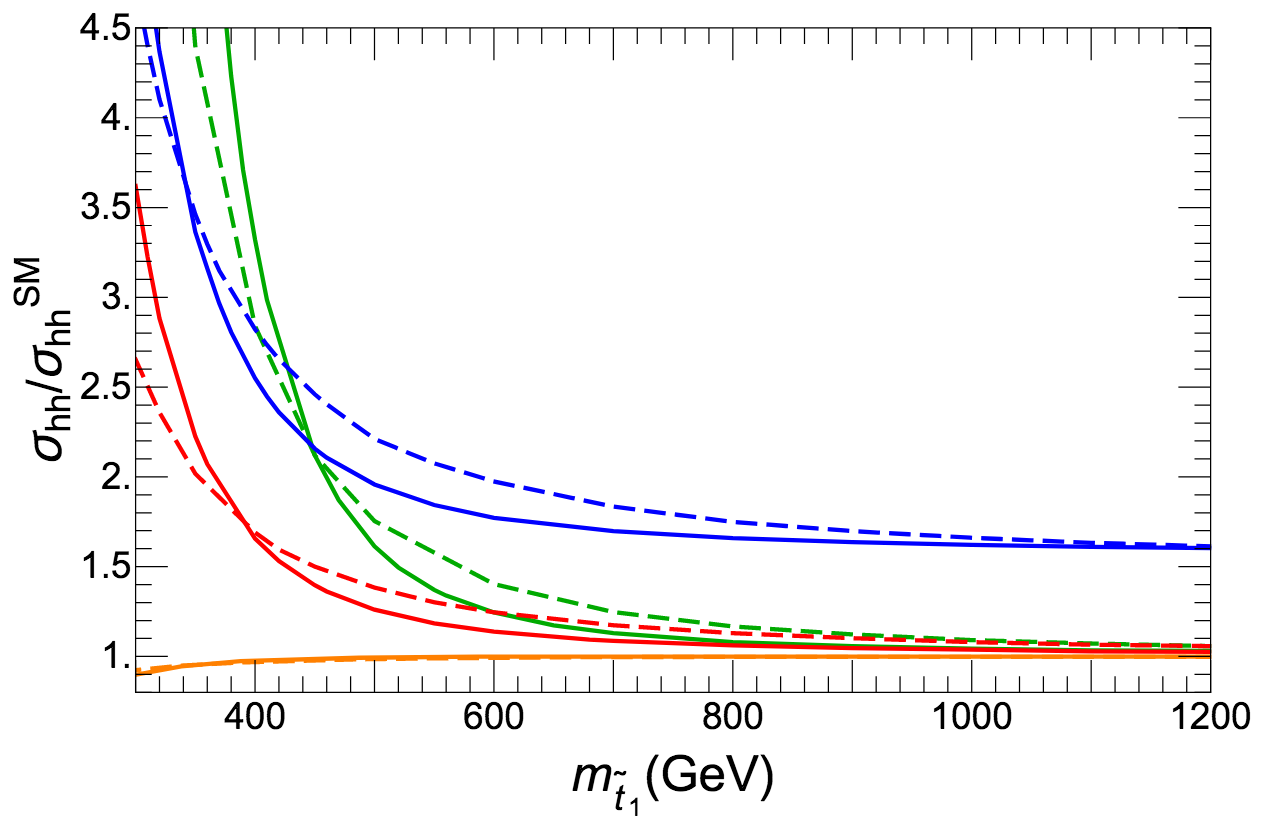
\includegraphics[width=0.65\textwidth]{figures/higgs_corr/sigma_hh_stops}
        \caption{
            Higgs pair production cross-section normalized to the SM prediction as a function
            of the mass of the lighter stop quark, $\tilde{t}_1$.
            Details in Ref.~\cite{LightStopsHiggs}.
        }
        \label{fig:hh_sigma_stops}
    \end{center}
\end{figure}

